\documentclass{beamer}
%\usetheme{boxed}

\usepackage{ae}
\usepackage{lmodern}

\definecolor{nesrocolor}{RGB}{200,200,255}
\setbeamertemplate{background canvas}[vertical shading][bottom=white,top=nesrocolor]

\setbeamercolor{structure}{fg=black}
\setbeamercolor{title}{fg=black}
\setbeamercolor{titlelike}{fg=black}
\setbeamercolor{section in sidebar}{fg=black}
\setbeamercolor{section in sidebar shaded}{fg=black}

\useinnertheme{default}


\newcommand{\backupbegin}{
   \newcounter{finalframe}
   \setcounter{finalframe}{\value{framenumber}}
}
\newcommand{\backupend}{
   \setcounter{framenumber}{\value{finalframe}}
}


\setbeamertemplate{footline}
{
  \leavevmode
  \hbox{
  \begin{beamercolorbox}[wd=1.0\paperwidth,ht=2.25ex,dp=2ex,center]{author in head/foot}%
    %\usebeamerfont{author in head/foot} Tomas Nesrovnal, FIT CVUT
Tom{\'{a}}\v{s} Nesrovnal $|$ Vliv form{\'{a}}tu ulo\v{z}en{\'{i}} \v{r}{\'{i}}dk{\'{e}} matice na v{\'{y}}konnost n{\'{a}}soben{\'{i}} \v{r}{\'{i}}dk{\'{y}}ch matic $|$ \insertframenumber{} / \inserttotalframenumber\hspace*{2ex}
  \end{beamercolorbox}
  }
  \vskip0pt%
}
\makeatother

%gets rid of some non important things
\setbeamertemplate{navigation symbols}{}
\setbeamercolor{separation line}{}

\usepackage{ucs}
\usepackage[utf8x]{inputenc}
\usepackage[czech]{babel}
\usepackage{palatino}
\usepackage{graphicx}

\author{Tomáš Nesrovnal}
\title{Vliv formátu uložení řídké matice na výkonnost násobení řídkých matic}
\institute{Fakulta informačních technologií\\České vysoké učení technické v Praze\\Obor: Teoretická informatika\\Vedoucí práce: Ing.~Ivan Šimeček,~Ph.D.}

\begin{document}

%%%%%%%%%%%%%%%%%%%%%%%%%%%%%%%%%%%%%%%%%%%%%%%%%%%%%%%%%%%%%%%%%%%%%%%%%%%%%%%%

\frame{
\titlepage
}

\frame{
	\begin{exampleblock}{Vliv formátu uložení řídké matice na výkonnost násobení řídkých matic}
		\begin{itemize}
			\item Nastudujte formáty uložení řídkých matic COO, CSR, BSR, Quadtree a algoritmy pro násobení matic v těchto formátech.
			\item Navrhněte modifikaci formátu Quadtree snížením výšky stromu, listy budou tvořeny podmaticemi ve formátu husté matice nebo ve formátech COO, CSR, BSR.
			\item V jazyce C implementujte algoritmy násobení matice vektorem a matice maticí ve formátech COO, CSR, BSR, Quadtree, modifikovaný formát Quadtree.
			\item Odvoďte jejich časové a paměťové složitosti, porovnejte tyto teoretické předpoklady s výkonností a paměťovými nároky jednotlivých implementací.
		\end{itemize}
	\end{exampleblock}
}

%%%%%%%%%%%%%%%%%%%%%%%%%%%%%%%%%%%%%%%%%%%%%%%%%%%%%%%%%%%%%%%%%%%%%%%%%%%%%%%%

%\section*{Obsah}
%\frame{
%	\frametitle{Obsah prezentace}
%	\tableofcontents
%}

%%%%%%%%%%%%%%%%%%%%%%%%%%%%%%%%%%%%%%%%%%%%%%%%%%%%%%%%%%%%%%%%%%%%%%%%%%%%%%%%	

\section{}

%%%%%%%%%%%%%%%%%%%%%%%%%%%%%%%%%%%%%%%%%%%%%%%%%%%%%%%%%%%%%%%%%%%%%%%%%%%%%%%%	

\section{Formáty řídkých matic}
\begin{frame}
	\frametitle{Formáty řídkých matic}
	\begin{itemize}
		\item COO -- uložení prvků
		\item CSR -- uložení řídkých řádků
		\item BSR -- uložení hustých bloků v řídkých řádcích
		\item Quadtree -- uložení bloků jako matice do listů kvadrantového stromu 
	\end{itemize}
\end{frame}
\section{Formát: k-ární strom}
\begin{frame}
	\frametitle{Formát: k-ární strom}
	\begin{exampleblock}{Nový formát}
		\begin{itemize}
			\item Zobecnění Quadtree na k-ární strom
			\item Listy tvořeny hustou, nebo CSR maticí
			\item Použit $2^2$-ární, $4^2$-ární a $8^2$-ární strom
		\end{itemize}
	\end{exampleblock}
\end{frame}
\begin{frame}
	\frametitle{Formát: k-ární strom}
	\begin{exampleblock}{Výhody}
		\begin{itemize}
			\item Snížení výšky stromu -- menší počet dereferencí ukazatelů
			\item Rozdělení bloků na husté a řídké
		\end{itemize}
	\end{exampleblock}
	\begin{alertblock}{Nevýhody}
		\begin{itemize}
			\item Náročnější implementace -- protože násobení matic není komutativní, je pro násobení hustých a~řídkých bloků spolu s vektorem potřeba celkem 6 (obecně $n*(n-1)$) funkcí
			\item Pamě\v{t}ové nároky na strukturu stromu
		\end{itemize}
	\end{alertblock}
\end{frame}
\begin{frame}
	\frametitle{Formát: k-ární strom}
	\begin{exampleblock}{Implementace}
		\begin{itemize}
			\item Jazyky C99, BASH
			\item Dvou-průchodové načítání matice (cachování bloků)
			\item V uzlech stromu pouze ukazatele do velkých polí
		\end{itemize}
	\end{exampleblock}
	\begin{exampleblock}{Testování}
		\begin{itemize}
			\item Funkčnost implementace byla otestována na mezních hodnotách, hustých maticích a maticemi z kolekce
			\item Matice vynásobeny algoritmem pro husté matice i~algoritmy pro řídké formáty a~výsledky s~tolerancí porovnány
		\end{itemize}
	\end{exampleblock}

\end{frame}
%%%%%%%%%%%%%%%%%%%%%%%%%%%%%%%%%%%%%%%%%%%%%%%%%%%%%%%%%%%%%%%%%%%%%%%%%%%%%%%%

\section{Měření}

%%==============================================================================

\subsection{Výběr z testovacích matic}
\begin{frame}
	\frametitle{Výběr z testovacích matic}
	
	\begin{table}[H]
	   \begin{tabular}{llllll}
	    Název matice & Velikost & Nenulových prvků            & Oblast                  \\
	    \hline
	    exdata\_1   &  6001    & 2.269500 $\cdot 10^6$ & optimalizace \\
	    human-gene2 & 14340    & 1.8068388 $\cdot 10^7$ & graf         \\
	    \end{tabular}
	\end{table}		
	
	\begin{figure}
		\centering
		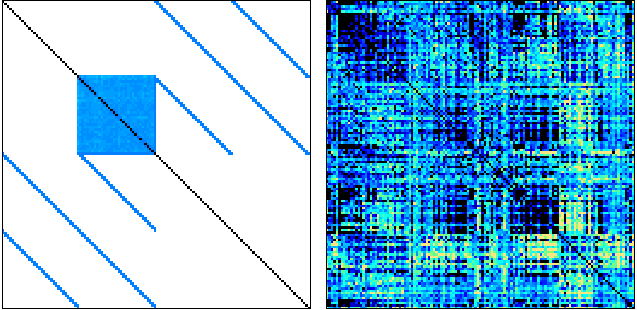
\includegraphics[width=1.0\textwidth]{./images/mtxs2}
		\caption{exdata\_1, human\_gene2}
	\end{figure}	
\end{frame}

\subsection{Násobení matice maticí}
\begin{frame}
	\frametitle{Měření: násobení matice maticí}
	
	\begin{figure}
		\centering
		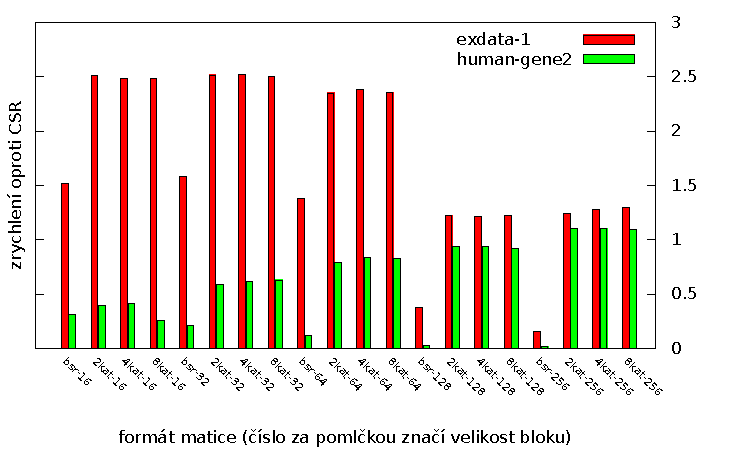
\includegraphics[width=1.0\textwidth]{./images/mmms2}
		%\caption{}
	\end{figure}	
\end{frame}

%%%%%%%%%%%%%%%%%%%%%%%%%%%%%%%%%%%%%%%%%%%%%%%%%%%%%%%%%%%%%%%%%%%%%%%%%%%%%%%%

\begin{frame}
	\begin{exampleblock}{Vliv formátu uložení řídké matice na výkonnost násobení řídkých matic}
		\begin{itemize}
			\item[\checkmark] Nastudujte formáty uložení řídkých matic COO, CSR, BSR, Quadtree a algoritmy pro násobení matic v těchto formátech.
			\item[\checkmark] Navrhněte modifikaci formátu Quadtree snížením výšky stromu, listy budou tvořeny podmaticemi ve formátu husté matice nebo ve formátech COO, CSR, BSR.
			\item[\checkmark] V jazyce C implementujte algoritmy násobení matice vektorem a matice maticí ve formátech COO, CSR, BSR, Quadtree, modifikovaný formát Quadtree.
			\item[\checkmark] Odvoďte jejich časové a paměťové složitosti, porovnejte tyto teoretické předpoklady s výkonností a paměťovými nároky jednotlivých implementací.
		\end{itemize}
	\end{exampleblock}
\end{frame}


%\begin{frame}
%	\frametitle{Děkuji za pozornost}
%	\begin{exampleblock}{Shrnutí}
%		\begin{itemize}
%			\item Formáty COO, CSR, BSR, Quadtree
%			\item Zobecnění formátu Quadtree, husté a řídké listy
%		\end{itemize}
%	\end{exampleblock}
%\end{frame}

%%%%%%%%%%%%%%%%%%%%%%%%%%%%%%%%%%%%%%%%%%%%%%%%%%%%%%%%%%%%%%%%%%%%%%%%%%%%%%%%


%\appendix
\backupbegin

\section{Otázky: oponent}
\begin{frame}
	\frametitle{Otázky: oponent (1/3)}
	\begin{exampleblock}{}
		\begin{itemize}
			\item Jakým způsobem byl měřen výpočetní čas při provádění experimentů?
			\item Byla do něj započítána i doba načítání matic?
			\item Jak byl proveden výpočet zrychlení oproti baseline formátu?
		\end{itemize}
	\end{exampleblock}
	\begin{alertblock}{}
	   \begin{itemize}
			\item Výpočetní čas byl měřen pomocí funkce \texttt{omp\_get\_wtime()} z knihovny OpenMP.
			\item Doba načítání matic (načítání ze souboru a převod do formátu) započítána nebyla.
			\item $$ speedup = \frac{mul\_time\_baseline\_format}{mul\_time\_format} $$
		\end{itemize}
	\end{alertblock}	
\end{frame}
\begin{frame}
	\frametitle{Otázky: oponent (2/3)}
	\begin{exampleblock}{}
		\begin{itemize}
			\item Byla měření prováděna opakovaně a byly výsledky průměrovány, anebo se jednalo o jednorázová měření?
		\end{itemize}
	\end{exampleblock}
	\begin{alertblock}{}
	   \begin{itemize}
			\item Násobení matice maticí provedeno jednou.
			\item Násobení matice vektorem provedeno stokrát, časy byly sečteny, neprůměrovány.
		\end{itemize}
	\end{alertblock}	
\end{frame}
\begin{frame}
	\frametitle{Otázky: oponent (3/3)}
	\begin{exampleblock}{}
		\begin{itemize}
			\item Veškeré experimenty jsou provedeny pouze na čtvercových maticích. Podporuje Vaše implementace i~obecné, obdélníkové
matice?
		\end{itemize}
	\end{exampleblock}
	\begin{alertblock}{}
	   \begin{itemize}
			\item Implementace s~maticemi typu $(m,n)$ pracuje jako s~maticemi typu $(max(m,n),max(m,n))$.
			\item Formát Quadtree a k-ární strom jsou ze své podstaty obdélníkové matice.
		\end{itemize}
	\end{alertblock}	
\end{frame}

\section{Otázky: vedoucí}
\begin{frame}
	\frametitle{Otázky: vedoucí (1/1)}
	\begin{exampleblock}{}
		\begin{itemize}
			\item Proč byla zvolena tak veliká hodnota parametru pro formát BSR?
		\end{itemize}
	\end{exampleblock}
	\begin{alertblock}{}
	   \begin{itemize}
			\item Měření byla provedena pro všechny blokové formáty pro velikosti bloků $2^k, k \in \{1,2,3,\ldots,8\}$.
			\item Násobení matice maticí ve formátu BSR obsahuje šest for cyklů. Velikosti bloků 2,4 a 8 jsou tak malé, že měření ukázala velmi slabý výkon. Z tohoto důvodu nebyla tato měření součástí grafů.
		\end{itemize}
	\end{alertblock}	
\end{frame}

\backupend

\end{document}
